\documentclass{standalone}% For the example only, any class will do

\usepackage{tikz}
\usetikzlibrary{positioning}% To get more advances positioning options
\usetikzlibrary{arrows}% To get more arrow heads
\usetikzlibrary{calc}
\begin{document}
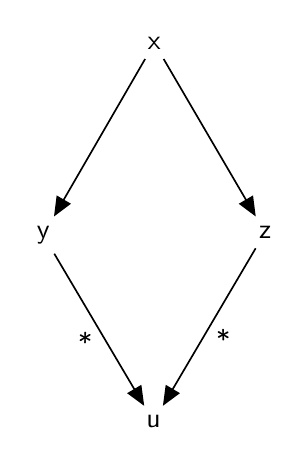
\begin{tikzpicture}[>=triangle 45,font=\sffamily]
    \node (X) at (0,0) {x};
    \node (Y) [below left=2cm and 1cm of X]  {y};% 2cm below, 1cm to the left (optional)
    \node (Z) [below right=2cm and 1cm of X] {z};
    \node (U) [below left=2cm and 1cm of Z]  {u};
    \draw [semithick,->] (X) -- (Y);
    \draw [semithick,->] (X) -- (Z);
    \draw [semithick,->] (Y) -- (U) node [midway,below,sloped] {*};
    \draw [semithick,->] (Z) -- (U) node [midway,below,sloped] {*};
\end{tikzpicture}
\end{document}
